\documentclass[journal]{IEEEtran}
\usepackage[margin=1in]{geometry}
\usepackage{amsmath,amssymb,booktabs,url,cite,tikz}
\usetikzlibrary{arrows.meta,positioning}
\usepackage{algorithm,algpseudocode}
\usepackage[hidelinks]{hyperref}
\newcommand{\T}{\mathsf T}
\begin{document}
\title{Recursive Probabilistic Estimation of Dynamic Graph Edge Weights from Node Signals}
\author{Gurui~Jin and Ercan~E.~Kuruo\u{g}lu%
\thanks{Gurui Jin and Ercan E. Kuruo\u{g}lu are with Shenzhen International Graduate School, Tsinghua University, Shenzhen, China (e-mail: jgr23@mails.tsinghua.edu.cn; kuruoglu@sz.tsinghua.edu.cn).}}
\maketitle
\begin{abstract}
Dynamic graph tracking requires estimating both the existence and strength of edges. We study recursive probabilistic estimation of dynamic edge weights from node signals. Node dynamics yield an edge-weight regression; Markov prediction and mean-field updating maintain edge probabilities. A support decision followed by conditional amplitude estimation produces a Laplacian and its complete spectrum. On 24 synthetic condition trajectories comprising 1,728 blocks, mean relative edge-weight and eigenvalue errors decrease from 0.15134 and 0.08741 for a task-adapted hard-threshold sparse EKF to 0.12163 and 0.06527. False splits of connected graphs decrease from 76/1068 to 8/1068. These improvements come with greater computation time and worse event-block increment error. We evaluate this tradeoff through the structural, weight, and spectral outputs of a single estimator.
\end{abstract}
\begin{IEEEkeywords}
Dynamic graph learning, edge-weight estimation, recursive inference, mean-field approximation, graph spectra.
\end{IEEEkeywords}
\section{Introduction}
\IEEEPARstart{G}{raph} signal processing describes interactions between nodes and uses Laplacian spectra to characterize signal variation \cite{shuman}. When edges disappear, reappear, and change strength, online inference must distinguish absent edges from weak connections while tracking their amplitudes. We ask how observed node trajectories, under a specified interaction model, can provide recursive edge estimates and consistent spectral outputs $U_t,\Lambda_t$.

Natali \emph{et al.} study time-varying optimization for online graph learning \cite{natali}. Dabush \emph{et al.} treat edge weights as latent states and graph-filtered signals as observations in a sparsity-aware EKF \cite{dabush}. Edge-weight Laplacian parameterization and the linear special case of first-order graph filtering are established foundations. Our coordinate update likewise uses standard mean-field variational inference \cite{blei}.

\textbf{The estimator constructs an edge-weight likelihood from successive node observations, recursively maintains a discrete distribution for each edge, and uses it to estimate connections and their strengths.} It combines Markov prediction, mean-field updating, and a point-estimate readout. Distributions carry information from one block to the next. We evaluate estimation error, structural recovery, and computational cost against literature-derived baselines.

\section{From Node Observations to Edge Information}
\subsection{Unknowns, observations, and modeling rationale}
Let $s_{t,k}\in\mathbb R^n$ contain scalar node signals. Index $t$ denotes a graph-update block and $k$ a within-block sample. The unknown $\theta_t\in[0,1]^m$ contains candidate \emph{edge} weights, not node values. Each column of $B=[b_1,\ldots,b_m]$ has $+1,-1$ at the endpoints of one edge and zeros elsewhere, giving
\begin{equation}
L(\theta_t)=B\operatorname{diag}(\theta_t)B^\T.\label{eq:lap}
\end{equation}
The arbitrary orientation does not affect $b_eb_e^\T$.
We use the first-order local interaction model
\begin{equation}
s_{t,k+1}=(aI-\eta L(\theta_t))s_{t,k}+u_{t,k}+\epsilon_{t,k}.\label{eq:dynamic}
\end{equation}
At node $i$, the interaction is $-\eta\sum_j\theta_{ij}(s_{i,k}-s_{j,k})$, added to self-evolution $as_{i,k}$ and known input $u_{i,k}$. This discrete diffusion-type graph filter \cite{shuman} applies when signals follow such coupling. All states are synchronously observed; $a,\eta,u,\sigma$ are known. Process innovations are independent across transitions, independent of the current state, and distributed as $\mathcal N(0,\sigma^2I)$. There is no additional sensor measurement noise.

For intuition, consider room temperatures coupled by heat exchange. Edge weights describe exchange strengths, while $as+u$ predicts the next temperatures without inter-room exchange. The difference from the observed next temperatures contains coupling and disturbance. Repeated temperature changes therefore inform the unknown strengths. 

\subsection{Residual meaning and derivation}
The regression response is computed from observations:
\begin{equation}
r_{t,k}=as_{t,k}+u_{t,k}-s_{t,k+1}.\label{eq:r}
\end{equation}
Here $s_{t,k}$ is the current observed node-signal vector; $a$ is the known self-evolution coefficient; $as_{t,k}$ predicts self-evolution alone; $u_{t,k}$ is the known input over the sampling interval; and $s_{t,k+1}$ is the next observation. Adding the first two terms predicts the next state without neighbor interactions. Subtracting the observation gives $r_{t,k}$. For a node with current value 1, $a=0.9$, input 0.02, and next observation 0.82, the residual is $0.9\times1+0.02-0.82=0.10$. It contains neighbor coupling and disturbance. Suppressing indices, substitution gives
\begin{align}
r&=as+u-[(aI-\eta L)s+u+\epsilon]\notag\\
 &=\eta Ls-\epsilon\notag\\
 &=\eta B\operatorname{diag}(\theta)B^\T s-\epsilon\notag\\
 &=\underbrace{\eta B\operatorname{diag}(B^\T s)}_{H}\theta-\epsilon.\label{eq:derive}
\end{align}
The last step uses $\operatorname{diag}(\theta)d=\operatorname{diag}(d)\theta$ for $d=B^\T s$. Column $e$ is $\eta b_e(b_e^\T s)$: an endpoint indicator scaled by the endpoint signal difference and coupling coefficient. Once $s$ is observed, $H$ is known and the equation is linear in $\theta$.

Before observation, the innovation and unknown weights make the next state and residual random. After observation, the residual is numerically determined. These statements are compatible: the likelihood describes how the observed value depends on unknown weights. Edge estimation combines the interaction model with information from successive state transitions.

\subsection{Three-node example and block stacking}
For candidate edges $(1,2),(1,3),(2,3)$, take $s=(1,0,0.5)^\T$, $a=0.9$, $\eta=0.1$, and $u=0$. Then
\begin{equation}
B=\begin{bmatrix}1&1&0\\-1&0&1\\0&-1&-1\end{bmatrix},\quad
H=\begin{bmatrix}.1&.05&0\\-.1&0&-.05\\0&-.05&.05\end{bmatrix}.
\end{equation}
For example, the second column is $0.1(1,0,-1)^\T(1-0.5)$. Generating a noiseless example with $\theta=(0.8,0.5,0)^\T$ gives $H\theta=(.105,-.08,-.025)^\T$ and $s_{k+1}=(.795,.08,.475)^\T$. An observer computes the same residual as $0.9s-s_{k+1}$ without knowing the generating weights. Further within-block observations supply more equations for the same edge weights.

Keeping $\theta_t$ fixed for $K$ transitions provides $K$ equations. Stacking places them vertically, without averaging:
\begin{equation}
\underbrace{\begin{bmatrix}r_{t,0}\\\vdots\\r_{t,K-1}\end{bmatrix}}_{r_t\in\mathbb R^{nK}}
=\underbrace{\begin{bmatrix}H_{t,0}\\\vdots\\H_{t,K-1}\end{bmatrix}}_{H_t\in\mathbb R^{nK\times m}}\theta_t-\epsilon_t.\label{eq:stack}
\end{equation}
Each transition adds constraints on the same weights. Equal endpoint signals give $B^\T s=0$ and $H=0$, conveying no instantaneous edge information. Full column rank of the stacked design suffices for uniqueness of unconstrained noiseless regression; a prior does not replace missing observation information.

\section{Recursive Edge-Distribution Estimation}
\subsection{Finite representation and prediction}
Each edge takes values $v_j=j/64$, $j=0,\ldots,64$, with approximate probabilities $q_{t,e}(j)$. Here $v_0=0$ means no edge, while positive values describe connection strengths. Prediction is
\begin{equation}
p^-_{t,e}(j)=\sum_{i=0}^{64}q_{t-1,e}(i)T_{ij},\label{eq:predict}
\end{equation}
where $T_{ij}$ describes a transition between weight states. The experiments fix zero-to-positive and positive-to-zero switching probabilities to 0.01 per block, using a discretized Gaussian transition for positive amplitudes. The first block uses the initial distribution with zero-state probability 0.5; subsequent blocks each perform one prediction.

\subsection{Why mean-field, and how it updates}
Exact enumeration requires $65^m$ joint configurations. The factorization $q_t(\theta_t)=\prod_e q_{t,e}(\theta_{t,e})$ stores $65m$ probabilities. Interactions enter each update through current means, trading a general representation of inter-edge dependence for tractable computation \cite{blei}.

Multiplying the conditional transition densities along the observed trajectory yields the log likelihood
\begin{align}
\ell_t(\theta_t)&=-\tfrac12\theta_t^\T G_t\theta_t+h_t^\T\theta_t+C,\label{eq:like}\\
G_t&=H_t^\T H_t/\sigma^2,\quad h_t=H_t^\T r_t/\sigma^2.\notag
\end{align}
This sequential likelihood does not assume that the entire trajectory-dependent design is independent of all process innovations. Let $\mu_{t,f}=\sum_jv_jq_{t,f}(j)$. The standard rule $\log q_{t,e}=\log p^-_{t,e}+\mathbb E_{-e}\ell_t+\mathrm{const}$ gives
\begin{equation}
\begin{split}
q_{t,e}(j)&\propto p^-_{t,e}(j)\exp[-\tfrac12G_{t,ee}v_j^2+c_{t,e}v_j],\\
c_{t,e}&=h_{t,e}-\sum_{f\ne e}G_{t,ef}\mu_{t,f}.\label{eq:update}
\end{split}
\end{equation}
The cross term $-G_{ef}\theta_e\theta_f$ becomes $-G_{ef}v_j\mu_f$ after taking the expectation; terms independent of $v_j$ enter the normalizer. Updates use a fixed edge order, normalize each distribution, and stop when maximum mean and probability changes both fall below $10^{-8}$, or after 30 sweeps. Capped blocks are retained and recorded.

\subsection{One estimator and one point-output rule}
We fix the support readout
\begin{equation}
\hat\theta_{t,e}=\begin{cases}
0,&q_{t,e}(0)\geq1/2,\\
\displaystyle\frac{\sum_{j=1}^{64}v_jq_{t,e}(j)}{1-q_{t,e}(0)},&q_{t,e}(0)<1/2.
\end{cases}\label{eq:readout}
\end{equation}
This makes an existence decision followed by conditional amplitude estimation. For example, $q(0)=0.7$ produces zero instead of a small positive mixture mean. The output first decides existence, then estimates strength conditional on existence.

Equation~\eqref{eq:lap} then gives $\hat L_t$, and a full eigendecomposition yields $\hat L_t=\hat U_t\hat\Lambda_t\hat U_t^\T$. The recursive state is the edge distribution. Full EVD of the point graph produces $U,\Lambda$ as derived outputs for spectral-error evaluation; they do not enter the edge-distribution update.
\begin{figure}[t]
\centering
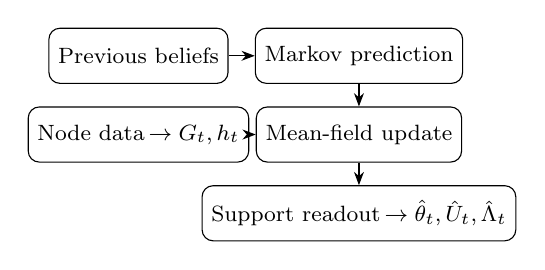
\begin{tikzpicture}[every node/.style={font=\footnotesize},box/.style={draw,rounded corners,align=center,minimum height=7mm},>=Stealth]
\node[box] (prior) at (0,0) {Previous beliefs};
\node[box] (pred) at (2.8,0) {Markov prediction};
\node[box] (data) at (0,-1.0) {Node data\,$\to G_t,h_t$};
\node[box] (upd) at (2.8,-1.0) {Mean-field update};
\node[box] (out) at (2.8,-2.0) {Support readout\,$\to\hat\theta_t,\hat U_t,\hat\Lambda_t$};
\draw[->] (prior)--(pred);\draw[->] (pred)--(upd);\draw[->] (data)--(upd);\draw[->] (upd)--(out);
\end{tikzpicture}
\caption{Prediction, observation update, and output of the estimator. Updated beliefs carry to the next block.}\label{fig:flow}
\end{figure}

\begin{algorithm}[t]
\caption{Recursive edge estimation from node signals}\label{alg:main}
\begin{algorithmic}[1]\footnotesize
\Require Node data, known $u,a,\eta,\sigma$, $B,T$, and initial beliefs
\For{each block $t$}
\State Use initial beliefs at the first block; otherwise predict by \eqref{eq:predict}
\State Form $r_t,H_t$ by \eqref{eq:r}, \eqref{eq:derive}, then $G_t,h_t$
\State Initialize $q$ from predicted beliefs and compute edge means
\For{at most 30 sweeps over edges in fixed order}
\State Update and normalize each $q_{t,e}$ by \eqref{eq:update}; refresh its mean
\State Stop after a sweep if probability and mean changes are both $\leq10^{-8}$
\EndFor
\State Read out $\hat\theta_t$ by \eqref{eq:readout}; retain $q_t$ for the next block
\State Form $\hat L_t$; output $\hat U_t,\hat\Lambda_t$ by full EVD
\EndFor
\end{algorithmic}\end{algorithm}

\subsection{Relationship to existing filters}
Our estimator and KF share Bayesian prediction and updating. Gaussian KF represents a continuous state by its mean and covariance; here, an explicit zero mass and positive grid probabilities are updated using~\eqref{eq:update}. Gaussian process innovations do not imply a single Gaussian edge posterior. The distinction is not observation nonlinearity:~\eqref{eq:derive} is exactly linear in edge weights and needs no EKF Taylor approximation. Dabush \emph{et al.} also address more general nonlinear graph filters \cite{dabush}.

\section{Experiments and Existing-Method Comparisons}
\subsection{Common task and metrics}
We use 6/12 nodes, two structural-change generators, two excitation conditions, and three graph draws per condition: 24 trajectories of 72 blocks, each with $K=48$ transitions. All $m=n(n-1)/2$ candidate edges are available. Parameters are $a=0.95$, $\eta=0.8/n$, and $\sigma=0.03$, with zero-mean Gaussian input standard deviation 0 or 0.3. Graph and observation seeds were fixed before testing; estimator parameters carry over from development. Paired excitation conditions share graphs, so the 1,728 blocks are not independent replicates.

\textbf{Literature-derived baselines.} The main comparison adapts the hard-threshold branch of the public implementation accompanying Dabush \emph{et al.} \cite{dabush,code} to the same regression, with $[0,1]$ constraints and the previously selected threshold 0.1. We call it the sparse EKF adaptation, distinguishing it from the paper's principal $\ell_1$ algorithm. The supplementary ProbSSM baseline comes from the same authors' repository \cite{code}. It maintains node-local binary incident-edge configurations with fixed positive amplitude 1. Its average and local-MAP readouts share inference. It is a repository baseline, not another proposed method or a substitute for the paper's main algorithm.

Every method accesses the same observed signals and known parameters, and computes a full spectrum from its point graph. For ascending eigenvalues $\lambda_t$, blockwise errors are
\begin{equation}
\begin{aligned}
E_\theta(t)&=\frac{\|\hat\theta_t-\theta_t\|_2}{\max(\|\theta_t\|_2,10^{-15})},\\
E_\lambda(t)&=\frac{\|\hat\lambda_t-\lambda_t\|_2}{\max(\|\lambda_t\|_2,10^{-15})}.
\end{aligned}
\end{equation}
We report means across blocks. Correct partition recovery requires all connected components to match on a disconnected true graph. A false split occurs when a connected true graph is estimated as disconnected. Their denominators are 660 and 1068 blocks, respectively. Components use strictly positive edges in the point graph.

\subsection{Accuracy, change error, and cost}
\begin{table}[t]
\caption{Same-observation graph estimation. Lower errors and false splits are better; more correct partitions are better. Column-wise best values are bold.}\label{tab:main}
\centering\scriptsize\setlength{\tabcolsep}{3pt}
\begin{tabular}{lrrrr}\toprule
Method & $E_\theta$ & $E_\lambda$ & Partitions & False splits\\\midrule
Proposed & \textbf{.12163} & \textbf{.06527} & 404/660 & 8/1068\\
Sparse EKF adapted & .15134 & .08741 & 330/660 & 76/1068\\
ProbSSM average & .16894 & .08844 & 2/660 & \textbf{0/1068}\\
ProbSSM local MAP & .19677 & .10135 & \textbf{545/660} & 103/1068\\\bottomrule
\end{tabular}
\end{table}
Relative to the sparse EKF adaptation, mean edge and eigenvalue errors decrease by about 19.6\% and 25.3\%, with improved aggregate partition counts. ProbSSM local MAP recovers more disconnected partitions but produces more false splits. ProbSSM was added on previously used observations; its fixed amplitude mismatches multivalued true weights, and its parameters were not independently optimized.

For blocks with true support changes, we average squared point-increment errors over all edges and event blocks, then take the square root. The proposed method scores 0.11435 versus 0.09379 for the sparse EKF adaptation: improved average estimation does not also improve abrupt-change response. Single-thread online time, including statistics, inference, and full EVD, averages 9.75 versus 1.04 seconds per trajectory. Initialization, warmup, storage, and evaluation are excluded; the machine was shared. All 14/1728 capped proposed-method blocks remain in the results. 

Under the archived common-gap selection, projection errors over 5,517 positive simple eigenvalue directions average 0.86552 (proposed) and 0.87621 (sparse EKF adaptation). Eligibility depends on truth and all outputs of the original experiment, excludes repeated eigenspaces, and does not establish a general advantage for the complete $U$.

\subsection{Synthetic UAV altitude coordination}
Consider high-level altitude coordination of six UAVs, with $s_i=z_i-z_{\rm ref}$ denoting deviation from a 30-m reference altitude. A first-order altitude response with neighbor consensus feedback \cite{consensus}, discretized by Euler with $\Delta=0.1$ s, gives
\begin{equation}
\begin{split}
s_{i,k+1}&=(1-\kappa\Delta)s_{i,k}+u_{i,k}+\epsilon_{i,k}\\
&\quad-c\Delta\sum_j\theta_{ij}(s_{i,k}-s_{j,k}).
\end{split}
\end{equation}
Set $\kappa=0.5$ and $c\Delta=0.8/6$, recovering \eqref{eq:dynamic}. The input $u_i$ is a known altitude-control increment and edge weights are effective neighbor-feedback strengths. Prescribed horizontal trajectories are held fixed within each block. Horizontal distance in meters sets $\theta_{ij}=\mathbf1[d_{ij}<35]\exp[-(d_{ij}/25)^2]$. Estimators receive only altitude signals, inputs, and known parameters.

Six new geometry seeds, 720110--720115, each use input standard deviations 0 and 0.3: 12 trajectories of 36 blocks, 432 blocks in total, with 48 transitions per block. Estimator parameters remain unchanged. The two input conditions share geometry; all 3/432 capped proposed-method blocks are retained. All nodes are observed synchronously under an ideal first-order altitude response. Table~\ref{tab:uav} reports this synthetic-model experiment.

\begin{table}[t]\centering\scriptsize
\caption{Synthetic high-level UAV model: relative errors and time.}\label{tab:uav}
\setlength{\tabcolsep}{4pt}\begin{tabular}{llrrr}\toprule
Input std. & Method & $E_\theta$ & $E_\lambda$ & ms/block\\\midrule
0 & Proposed & \textbf{.33687} & \textbf{.11018} & 2.92\\
0 & Sparse EKF & .39423 & .15612 & \textbf{.56}\\
0.3 & Proposed & \textbf{.07065} & \textbf{.02180} & 3.30\\
0.3 & Sparse EKF & .09069 & .03621 & \textbf{.59}\\\bottomrule
\end{tabular}\end{table}

To evaluate decision use, each block's same terminal state $s$ is supplied to controllers using the proposed estimate, the sparse EKF estimate, no graph, and the true graph. Minimizing predicted altitude error plus control effort gives $v=\operatorname{clip}(-\hat F s/2,-1,1)$, with $\hat F=aI-\eta\hat L$; the no-graph model uses $aI$. A shared true model and disturbance $w$ score $J=\|Fs+v+w\|^2+\|v\|^2$. With input standard deviation 0.3, mean costs are 0.701610, 0.701721, 0.745394, and 0.701512, respectively. The proposed estimate reduces cost by 5.87\% relative to no graph, but only 0.016\% relative to sparse EKF. With zero input, costs are 0.011256, 0.011258, 0.011698, and 0.011236. This is matched-state one-step decision replay: actions do not feed subsequent observations. The spectral expression $\hat F=\hat U(aI-\eta\hat\Lambda)\hat U^\T$ is equivalent to direct use of $\hat L$; the experiment evaluates use of the estimated graph.

\section{Conclusion}
The estimator constructs an edge-weight regression from successive node observations and recursively maintains edge distributions through Markov prediction and mean-field updating. It outputs dynamic connections and their strengths. In the original synthetic comparison, mean weight and eigenvalue errors decrease by 19.6\% and 25.3\% relative to the sparse EKF adaptation, while false splits decrease from 76/1068 to 8/1068, with greater computational cost and event-increment error. The added altitude-coordination simulation also yields lower average estimation errors; its one-step control cost is close to sparse EKF. These results characterize the estimator's accuracy, cost, and dynamic-response tradeoff.

\begin{thebibliography}{9}
\bibitem{shuman} D. I. Shuman, S. K. Narang, P. Frossard, A. Ortega, and P. Vandergheynst, ``The emerging field of signal processing on graphs: Extending high-dimensional data analysis to networks and other irregular domains,'' \emph{IEEE Signal Process. Mag.}, vol. 30, no. 3, pp. 83--98, 2013.
\bibitem{natali} A. Natali, E. Isufi, M. Coutino, and G. Leus, ``Learning time-varying graphs from online data,'' \emph{IEEE Open J. Signal Process.}, 2022, doi: 10.1109/OJSP.2022.3178901.
\bibitem{dabush} L. Dabush, N. Shlezinger, and T. Routtenberg, ``Sparsity-aware extended Kalman filter for tracking dynamic graphs,'' arXiv:2507.09999, 2025.
\bibitem{blei} D. M. Blei, A. Kucukelbir, and J. D. McAuliffe, ``Variational inference: A review for statisticians,'' \emph{J. Amer. Statist. Assoc.}, vol. 112, no. 518, pp. 859--877, 2017.
\bibitem{code} L. Dabush, ``PolyEKF,'' source snapshot cbb1a0a (full commit recorded with the experiments), \texttt{baseline\_prob\_ssm.py} and EKF implementation. [Online]. Available: \url{https://github.com/lital-dgold/PolyEKF}
\bibitem{consensus} R. Olfati-Saber and R. M. Murray, ``Consensus problems in networks of agents with switching topology and time-delays,'' \emph{IEEE Trans. Autom. Control}, vol. 49, no. 9, pp. 1520--1533, 2004, doi: 10.1109/TAC.2004.834113.
\end{thebibliography}
\end{document}

